\begin{figure}[hbt!]
    \centering
    \begin{subfigure}{0.2\textwidth}
        \centering
        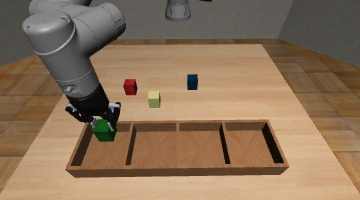
\includegraphics[width=\textwidth]{Figures/images/pick_place/task_1.png}
        \caption{First variation, green box into first bin}
        \label{fig:first_variation}
    \end{subfigure}
    \hfill
    \begin{subfigure}{0.2\textwidth}
        \centering
        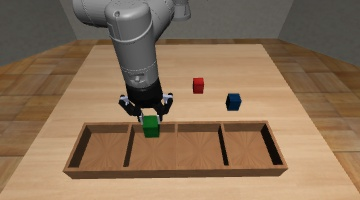
\includegraphics[width=\textwidth]{Figures/images/pick_place/task_2.png}
        \caption{Second variation, green box into second bin}
        \label{fig:second_variation}
    \end{subfigure}
    \hfill
    \begin{subfigure}{0.2\textwidth}
        \centering
        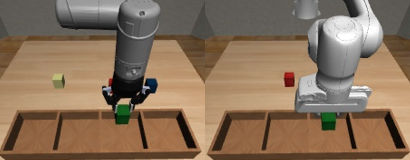
\includegraphics[width=\textwidth]{Figures/images/pick_place/task_3.png}
        \caption{Third variation, green box into third bin}
        \label{fig:third_variation}
    \end{subfigure}
    \hfill
    \begin{subfigure}{0.2\textwidth}
        \centering
        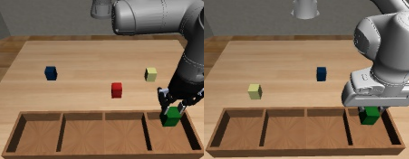
\includegraphics[width=\textwidth]{Figures/images/pick_place/task_4.png}
        \caption{Fourth variation, green box into fourth bin}
        \label{fig:fourth_variation}
    \end{subfigure}
    \caption{Example of variations for the Pick and Place task. The same set of variations is repeated for each block}
    \label{fig:example_of_variations_for_pick_place}
\end{figure}

\begin{figure}[hbt!]
    \centering
    \begin{subfigure}{0.2\textwidth}
        \centering
        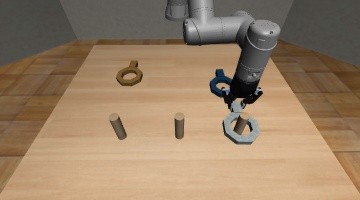
\includegraphics[width=\textwidth]{Figures/images/nut_assembly/task_1.png}
        \caption{First variation, assembly gray nut with right peg}
        \label{fig:first_variation_nut}
    \end{subfigure}
    \hspace{30px}
    \begin{subfigure}{0.2\textwidth}
        \centering
        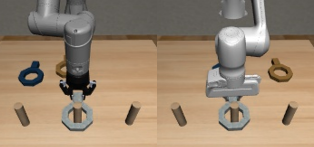
\includegraphics[width=\textwidth]{Figures/images/nut_assembly/task_2.png}
        \caption{Second variation, assembly gray nut with middle peg}
        \label{fig:second_variation_nut}
    \end{subfigure}
    \hspace{30px}
    \begin{subfigure}{0.2\textwidth}
        \centering
        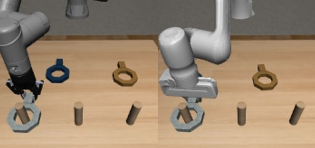
\includegraphics[width=\textwidth]{Figures/images/nut_assembly/task_3.png}
        \caption{Third variation, assembly gray nut with left peg}
        \label{fig:third_variation_nut}
    \end{subfigure}
    \caption{Example of variations for the Nut-Assembly. The same set of variations is repeated for each nut}
    \label{fig:examples_of_variations_for_nut_assembly}
\end{figure}